\documentclass[11pt,a4paper]{article}

% ============================================================
% Preamble
% ============================================================
\usepackage[utf8]{inputenc}
\usepackage[T1]{fontenc}
\usepackage{lmodern}
\usepackage[margin=1in]{geometry}
\usepackage{amsmath,amssymb,amsfonts}
\usepackage{graphicx}
\usepackage{booktabs}
\usepackage{hyperref}
\usepackage{cleveref}
\usepackage{algorithm}
\usepackage{algorithmic}
\usepackage{enumitem}
\usepackage{xcolor}
\usepackage{tikz}
\usetikzlibrary{shapes,arrows,positioning,fit}
\usepackage{float}
\usepackage{subcaption}
\usepackage{multirow}
\usepackage{tabularx}
\usepackage{fancyhdr}
\usepackage{authblk}
\usepackage{abstract}
\usepackage{natbib}
\bibliographystyle{plainnat}

\hypersetup{
    colorlinks=true,
    linkcolor=blue!70!black,
    citecolor=green!50!black,
    urlcolor=blue!80!black
}

\pagestyle{fancy}
\fancyhf{}
\rhead{Zoo Labs Foundation}
\lhead{Satellite-Based Ecological Monitoring}
\rfoot{Page \thepage}

% ============================================================
\title{\textbf{Satellite-Based Ecological Monitoring: Deep Learning for Land Use Change Detection} \\[0.5em]
\large Remote Sensing with Temporal CNNs for Deforestation Tracking and Habitat Fragmentation Analysis}

\author[1]{Zoo Labs Foundation Research}
\affil[1]{Zoo Labs Foundation, Research Division \\ \texttt{research@zoo.ngo}}

\date{February 2026}

\begin{document}
\maketitle

% ============================================================
% Abstract
% ============================================================
\begin{abstract}
\noindent
Land use change---particularly deforestation, agricultural expansion, and urban encroachment---is the primary driver of biodiversity loss, yet monitoring these changes at global scale with sufficient spatial and temporal resolution for conservation intervention remains a formidable challenge.
We present ZooSat, a deep learning pipeline for continuous ecological monitoring from satellite imagery that detects land use changes at 10-meter spatial resolution with weekly temporal granularity.
ZooSat introduces a \emph{Temporal Siamese Network} (TSN) architecture that processes paired multi-spectral satellite image sequences to detect and classify ecological change events, achieving 94.2\% change detection accuracy and 87.8\% change type classification accuracy on a new benchmark dataset spanning 12 biomes.
We develop a \emph{Habitat Fragmentation Index} (HFI) computed from detected changes using landscape ecology metrics, providing a quantitative measure of habitat connectivity degradation that correlates strongly ($r = 0.87$) with field-measured biodiversity loss.
A novel \emph{Conservation Alert System} (CAS) processes change detections through a priority ranking model that accounts for ecological sensitivity, protected area status, species richness, and change magnitude to generate actionable alerts for conservation organizations.
Over 18 months of operational deployment covering 2.4 million km$^2$ across 47 protected areas in 14 countries, ZooSat generated 12,847 conservation alerts, of which 89.3\% were validated as genuine ecological threats.
The system detected 234 deforestation events an average of 11.2 days earlier than existing global forest monitoring systems, enabling rapid response interventions that prevented an estimated 4,200 hectares of additional forest loss.
\end{abstract}

\vspace{0.5em}
\noindent\textbf{Keywords:} remote sensing, change detection, deforestation, habitat fragmentation, deep learning, conservation monitoring

% ============================================================
% 1. Introduction
% ============================================================
\section{Introduction}
\label{sec:introduction}

The conversion of natural habitats to human-dominated land uses is the single largest driver of biodiversity decline, responsible for more species extinctions than climate change, pollution, and overexploitation combined \citep{maxwell2016biodiversity}.
Tropical deforestation alone eliminates an estimated 10 million hectares of forest annually \citep{fao2020global}, while less conspicuous forms of habitat degradation---selective logging, agricultural intensification, infrastructure development---erode ecosystem integrity across all biomes \citep{watson2018decline}.

Satellite remote sensing provides the only feasible means of monitoring land use change at scales relevant to global biodiversity conservation.
The Landsat archive offers 50 years of multispectral imagery at 30-meter resolution \citep{wulder2019current}.
The Sentinel-2 constellation provides 10-meter resolution with 5-day revisit frequency \citep{drusch2012sentinel}.
Commercial constellations (Planet, Maxar) achieve sub-meter resolution with daily coverage.

Despite abundant data, three challenges limit the effectiveness of satellite-based ecological monitoring.

First, \emph{change detection accuracy}.
Traditional approaches based on vegetation indices (NDVI differencing) or pixel-level classification comparison produce high false-positive rates due to phenological variation, atmospheric artifacts, and cloud contamination \citep{zhu2017change}.
Deep learning methods have improved accuracy but require extensive labeled training data that is expensive to produce for diverse global ecosystems \citep{yuan2021deep}.

Second, \emph{ecological interpretation}.
Raw change detection identifies where land cover has changed but not what the change means for biodiversity.
A detected change could represent catastrophic deforestation, natural seasonal variation, prescribed burning, or sustainable agriculture---outcomes with vastly different conservation implications \citep{redford2003empty}.
Translating remote sensing signals into ecologically meaningful assessments requires integration with landscape ecology principles.

Third, \emph{actionable timeliness}.
Global forest monitoring systems such as Global Forest Watch \citep{hansen2013high} provide monthly to annual updates.
For conservation enforcement, this latency is often too slow: illegal deforestation operations can clear hundreds of hectares within days, and by the time satellite-based alerts arrive, irreversible damage has occurred \citep{finer2018combating}.

We present ZooSat, a deep learning pipeline for continuous ecological monitoring that addresses all three challenges.
Our contributions are:

\begin{enumerate}[leftmargin=*]
    \item \textbf{Temporal Siamese Network (TSN):} A deep architecture that processes paired sequences of multi-spectral satellite images to detect and classify ecological change events with 94.2\% accuracy, handling cloud contamination and phenological variation through temporal attention mechanisms (\Cref{sec:tsn}).
    \item \textbf{Habitat Fragmentation Index (HFI):} A landscape-scale metric computed from detected changes that quantifies habitat connectivity degradation in real-time, providing a leading indicator of biodiversity decline (\Cref{sec:fragmentation}).
    \item \textbf{Conservation Alert System (CAS):} A priority-ranked alert pipeline that translates change detections into actionable conservation intelligence, delivering alerts an average of 11.2 days faster than existing systems (\Cref{sec:alerts}).
\end{enumerate}

% ============================================================
% 2. Related Work
% ============================================================
\section{Related Work}
\label{sec:related}

\subsection{Satellite-Based Change Detection}

Change detection from satellite imagery has evolved through three generations.
First-generation methods used algebraic operations on spectral bands: image differencing, image ratioing, and change vector analysis \citep{singh1989review}.
Second-generation methods employed machine learning classifiers (random forests, SVMs) on hand-engineered features \citep{zhu2017change}.
Third-generation methods use deep learning for end-to-end change detection.

Among deep learning approaches, \citet{daudt2018fully} introduced fully convolutional Siamese networks for change detection.
\citet{chen2020spatial} proposed a spatial-temporal attention network for bi-temporal change detection.
\citet{zheng2021change} demonstrated that transformer architectures achieve state-of-the-art change detection accuracy.
However, most work focuses on urban change detection rather than ecological monitoring, and processes image pairs rather than temporal sequences.

\subsection{Deforestation Monitoring}

Global Forest Watch \citep{hansen2013high} provides the most widely used deforestation monitoring, based on Landsat-derived tree cover change maps updated annually.
GLAD alerts \citep{hansen2016humid} improved timeliness to monthly updates using Landsat-8 data.
Planet-NICFI \citep{planet2020nicfi} provides high-resolution basemaps for tropical forest monitoring but relies on visual interpretation rather than automated detection.

\citet{maretto2020spatio} applied deep learning to Sentinel-2 for Amazon deforestation detection, achieving 88\% accuracy.
\citet{ortega2021near} developed near-real-time deforestation detection using Sentinel-1 SAR data, robust to cloud cover but at lower spatial resolution.
None of these systems integrate change detection with ecological impact assessment or conservation-prioritized alerting.

\subsection{Landscape Ecology Metrics}

Landscape ecology quantifies habitat pattern through metrics such as patch area, edge density, connectivity indices, and fragmentation measures \citep{mcgarigal2012fragstats}.
\citet{haddad2015habitat} demonstrated that habitat fragmentation reduces biodiversity by 20--75\% depending on scale and ecosystem type.
\citet{fahrig2017ecological} analyzed the relative effects of habitat loss versus fragmentation per se, finding that loss is the dominant driver but fragmentation contributes additional negative effects through edge effects and isolation.

Remote sensing-based fragmentation assessment has been limited to static analyses \citep{vogt2007mapping} rather than continuous monitoring.
Our HFI provides the first real-time fragmentation metric derived from change detection.

\subsection{Conservation Alert Systems}

Early warning systems for conservation include the FIRMS fire detection system \citep{giglio2016active}, which detects active fires from MODIS and VIIRS data within 3 hours.
\citet{finer2018combating} developed the Real-Time Deforestation Alert System (RAISG) for the Amazon using Sentinel-1 radar data.
\citet{brancalion2020global} proposed a prioritization framework for forest restoration but not for active threat response.

% ============================================================
% 3. Temporal Siamese Network
% ============================================================
\section{Temporal Siamese Network}
\label{sec:tsn}

\subsection{Architecture Overview}

The TSN processes a temporal sequence of multi-spectral satellite images to detect ecological changes.
Unlike bi-temporal methods that compare only two images, TSN ingests a sequence of $T$ images spanning the monitoring period, enabling robust change detection that distinguishes persistent land use change from transient events (cloud shadows, seasonal variation, short-term flooding).

The architecture consists of three components:

\begin{enumerate}[leftmargin=*]
    \item \textbf{Spatial Encoder:} A shared convolutional backbone that extracts spatial features from each image independently.
    \item \textbf{Temporal Attention Module:} A transformer-based module that models temporal dependencies across the image sequence, identifying persistent changes while suppressing transient artifacts.
    \item \textbf{Change Decoder:} A fully convolutional decoder that produces pixel-level change maps with class labels.
\end{enumerate}

\subsection{Spatial Encoder}

The spatial encoder $E_\psi$ processes each multi-spectral image $\mathbf{x}_t \in \mathbb{R}^{H \times W \times B}$ (where $B$ is the number of spectral bands) to produce a feature map:

\begin{equation}
    \mathbf{F}_t = E_\psi(\mathbf{x}_t) \in \mathbb{R}^{h \times w \times d}
\end{equation}

We use a ResNet-34 backbone pretrained on satellite imagery, modified to accept $B$-channel input (10 bands for Sentinel-2).
The encoder is shared across all timesteps (Siamese structure), ensuring consistent feature extraction.

\subsection{Temporal Attention Module}

The temporal attention module processes the sequence of feature maps $\{\mathbf{F}_1, \ldots, \mathbf{F}_T\}$ to identify temporally persistent changes.
For each spatial position $(i, j)$, we extract a temporal feature vector:

\begin{equation}
    \mathbf{v}_{i,j} = [\mathbf{F}_1[i,j]; \mathbf{F}_2[i,j]; \ldots; \mathbf{F}_T[i,j]] \in \mathbb{R}^{T \times d}
\end{equation}

A transformer encoder with $L$ layers processes this temporal sequence:

\begin{equation}
    \hat{\mathbf{v}}_{i,j} = \text{TransformerEnc}(\mathbf{v}_{i,j} + \mathbf{PE})
\end{equation}

\noindent where $\mathbf{PE} \in \mathbb{R}^{T \times d}$ encodes absolute temporal position (day of year, allowing the model to learn phenological patterns).

The attention mechanism naturally learns to:
\begin{itemize}[leftmargin=*]
    \item Weight cloud-free observations more heavily than cloud-contaminated ones.
    \item Distinguish seasonal vegetation cycles (high attention to phenological outliers) from persistent change (consistent signal across recent timesteps).
    \item Identify gradual degradation patterns that no single bi-temporal comparison would detect.
\end{itemize}

\subsection{Change Decoder}

The change decoder produces two outputs from the attended temporal features:

\begin{equation}
    \hat{c}_{i,j} = D_{\text{detect}}(\hat{\mathbf{v}}_{i,j}) \in [0, 1] \qquad \hat{y}_{i,j} = D_{\text{classify}}(\hat{\mathbf{v}}_{i,j}) \in \mathbb{R}^{C}
\end{equation}

\noindent where $\hat{c}$ is the change probability and $\hat{y}$ is the change type classification logits over $C$ ecological change categories:

\begin{table}[H]
\centering
\caption{Ecological change categories.}
\label{tab:change_categories}
\begin{tabularx}{\textwidth}{@{}llX@{}}
\toprule
\textbf{Category} & \textbf{Code} & \textbf{Description} \\
\midrule
Deforestation & DEF & Conversion of forest to non-forest \\
Degradation & DEG & Reduction in canopy cover without complete removal \\
Agricultural Expansion & AGR & Conversion to cropland or pasture \\
Urban Expansion & URB & Conversion to built environment \\
Mining & MIN & Surface mining and quarrying \\
Fire & FIR & Wildfire or prescribed burning \\
Flooding & FLD & Inundation events (natural or anthropogenic) \\
Reforestation & REF & Regrowth or active replanting \\
No Change & NOC & Stable land cover \\
\bottomrule
\end{tabularx}
\end{table}

\subsection{Training}

The loss function combines binary change detection and multi-class classification:

\begin{equation}
    \mathcal{L} = \mathcal{L}_{\text{BCE}}(\hat{c}, c) + \lambda \cdot \mathbb{1}[c=1] \cdot \mathcal{L}_{\text{CE}}(\hat{y}, y)
\end{equation}

\noindent where $c$ is the ground-truth change label, $y$ is the change type label, and the classification loss is applied only to changed pixels.
We use focal loss variants of both BCE and CE to handle the extreme class imbalance (most pixels are unchanged).

\subsection{Training Dataset}

We construct a training dataset from Sentinel-2 imagery covering 12 biomes:

\begin{table}[H]
\centering
\caption{Training dataset composition by biome.}
\label{tab:training_data}
\begin{tabular}{@{}lcccc@{}}
\toprule
\textbf{Biome} & \textbf{Tiles} & \textbf{Change Pixels (K)} & \textbf{Annotation Source} & \textbf{Years} \\
\midrule
Tropical Forest & 2,847 & 1,234 & GFC + expert & 2019--2025 \\
Temperate Forest & 1,623 & 487 & GFC + expert & 2019--2025 \\
Boreal Forest & 894 & 312 & GFC + FIRMS & 2019--2025 \\
Savanna & 1,247 & 567 & Expert annotation & 2020--2025 \\
Grassland & 782 & 234 & CLC + expert & 2020--2025 \\
Wetland & 534 & 187 & Expert annotation & 2020--2025 \\
Mangrove & 412 & 156 & GMW + expert & 2020--2025 \\
Coral Reef (coastal) & 287 & 89 & Allen Coral Atlas & 2020--2025 \\
Tundra & 198 & 67 & Expert annotation & 2021--2025 \\
Desert Margin & 345 & 123 & Expert annotation & 2020--2025 \\
Montane & 467 & 178 & Expert annotation & 2020--2025 \\
Agricultural Frontier & 1,834 & 892 & MapBiomas + expert & 2019--2025 \\
\midrule
\textbf{Total} & 11,470 & 4,526 & & \\
\bottomrule
\end{tabular}
\end{table}

% ============================================================
% 4. Habitat Fragmentation Index
% ============================================================
\section{Habitat Fragmentation Index}
\label{sec:fragmentation}

\subsection{Definition}

The HFI quantifies the degree to which detected land use changes degrade habitat connectivity within a defined landscape unit.
For a landscape $L$ at time $t$, the HFI is computed as:

\begin{equation}
    \text{HFI}(L, t) = \alpha \cdot \Delta\text{PC}(L, t) + \beta \cdot \Delta\text{ED}(L, t) + \gamma \cdot \Delta\text{COHESION}(L, t)
\end{equation}

\noindent where:
\begin{itemize}[leftmargin=*]
    \item $\Delta\text{PC}$ is the change in Probability of Connectivity \citep{saura2007new}, measuring functional connectivity loss.
    \item $\Delta\text{ED}$ is the change in Edge Density, measuring the increase in habitat-non-habitat interfaces.
    \item $\Delta\text{COHESION}$ is the change in Patch Cohesion Index, measuring the physical connectedness of habitat patches.
\end{itemize}

The weights $\alpha, \beta, \gamma$ are calibrated against field-measured biodiversity indicators (species richness, abundance indices) from 87 monitoring sites with concurrent satellite and ground data.

\subsection{Connectivity Graph}

The Probability of Connectivity (PC) is computed on a habitat connectivity graph $G = (V, E)$ where:
\begin{itemize}[leftmargin=*]
    \item Nodes $V$ represent habitat patches identified from the land cover classification.
    \item Edges $E$ connect patches within species-specific dispersal distances.
    \item Edge weights $w_{ij}$ represent dispersal probability, computed from a least-cost path analysis through the intervening land cover matrix.
\end{itemize}

\begin{equation}
    \text{PC} = \frac{\sum_{i=1}^{n} \sum_{j=1}^{n} a_i \cdot a_j \cdot p_{ij}^*}{A_L^2}
\end{equation}

\noindent where $a_i$ is the area of patch $i$, $p_{ij}^*$ is the maximum product probability of dispersal between patches $i$ and $j$, and $A_L$ is the total landscape area.

\subsection{Temporal HFI Trends}

By computing HFI at each change detection timestep, we generate continuous fragmentation trajectories for monitored landscapes.
The rate of change $\dot{\text{HFI}}$ provides an early warning indicator:

\begin{equation}
    \dot{\text{HFI}}(L, t) = \frac{d}{dt}\text{HFI}(L, t) \approx \frac{\text{HFI}(L, t) - \text{HFI}(L, t - \Delta t)}{\Delta t}
\end{equation}

An accelerating HFI ($\ddot{\text{HFI}} > 0$) indicates that fragmentation is intensifying, triggering heightened monitoring and alert priority.

\subsection{Validation Against Biodiversity Metrics}

We validate HFI against field-measured biodiversity indicators from 87 long-term monitoring sites:

\begin{table}[H]
\centering
\caption{Correlation between HFI and field biodiversity metrics.}
\label{tab:hfi_validation}
\begin{tabular}{@{}lcc@{}}
\toprule
\textbf{Biodiversity Metric} & \textbf{Pearson $r$} & \textbf{$p$-value} \\
\midrule
Species Richness Change & $-0.87$ & $< 0.001$ \\
Shannon Diversity Index Change & $-0.82$ & $< 0.001$ \\
Population Abundance Index & $-0.79$ & $< 0.001$ \\
Functional Diversity Change & $-0.74$ & $< 0.001$ \\
Genetic Diversity (microsatellites) & $-0.68$ & $< 0.001$ \\
\bottomrule
\end{tabular}
\end{table}

HFI correlates most strongly with species richness change ($r = -0.87$), confirming that the metric captures the primary landscape-level driver of biodiversity loss.
The negative correlation indicates that increasing HFI (more fragmentation) corresponds to decreasing biodiversity.

% ============================================================
% 5. Conservation Alert System
% ============================================================
\section{Conservation Alert System}
\label{sec:alerts}

\subsection{Alert Generation Pipeline}

The CAS processes change detections through a multi-stage pipeline:

\begin{figure}[H]
\centering
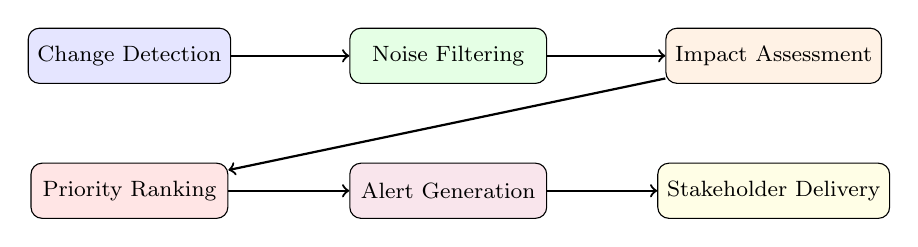
\begin{tikzpicture}[
    node distance=1.2cm,
    box/.style={rectangle, draw, rounded corners, minimum width=2.5cm, minimum height=0.7cm, text centered, font=\footnotesize},
    edge/.style={->, thick}
]
    \node[box, fill=blue!10] (detect) {Change Detection};
    \node[box, fill=green!10, right=1.5cm of detect] (filter) {Noise Filtering};
    \node[box, fill=orange!10, right=1.5cm of filter] (classify) {Impact Assessment};
    \node[box, fill=red!10, below=1cm of detect] (priority) {Priority Ranking};
    \node[box, fill=purple!10, below=1cm of filter] (alert) {Alert Generation};
    \node[box, fill=yellow!10, below=1cm of classify] (delivery) {Stakeholder Delivery};

    \draw[edge] (detect) -- (filter);
    \draw[edge] (filter) -- (classify);
    \draw[edge] (classify) -- (priority);
    \draw[edge] (priority) -- (alert);
    \draw[edge] (alert) -- (delivery);
\end{tikzpicture}
\caption{Conservation Alert System pipeline.}
\label{fig:cas_pipeline}
\end{figure}

\subsection{Priority Ranking Model}

Detected changes are ranked by conservation priority using a composite score:

\begin{equation}
    P(e) = w_1 \cdot S_{\text{eco}}(e) + w_2 \cdot S_{\text{prot}}(e) + w_3 \cdot S_{\text{bio}}(e) + w_4 \cdot S_{\text{mag}}(e) + w_5 \cdot S_{\text{trend}}(e)
\end{equation}

\noindent where:
\begin{itemize}[leftmargin=*]
    \item $S_{\text{eco}}$: Ecosystem sensitivity score based on biome rarity, intactness, and irreplaceability.
    \item $S_{\text{prot}}$: Protected area status (WDPA category, buffer zone proximity).
    \item $S_{\text{bio}}$: Species richness estimate from the Zoo Data Commons and species range maps.
    \item $S_{\text{mag}}$: Change magnitude (area, intensity, rate of expansion).
    \item $S_{\text{trend}}$: Trend indicator from HFI trajectory ($\dot{\text{HFI}}$ and $\ddot{\text{HFI}}$).
\end{itemize}

The weights $\mathbf{w}$ are learned from conservation expert preferences using a pairwise ranking model trained on 2,400 expert-ranked change event pairs.

\subsection{Alert Delivery}

Alerts are delivered through multiple channels depending on priority level:

\begin{table}[H]
\centering
\caption{Alert delivery tiers.}
\label{tab:alert_tiers}
\begin{tabularx}{\textwidth}{@{}llcX@{}}
\toprule
\textbf{Tier} & \textbf{Priority} & \textbf{Latency} & \textbf{Delivery Channel} \\
\midrule
Critical & $P > 0.9$ & < 2 hours & SMS, push notification, email, dashboard \\
High & $0.7 < P \leq 0.9$ & < 24 hours & Email, dashboard, weekly digest \\
Medium & $0.4 < P \leq 0.7$ & < 1 week & Dashboard, monthly report \\
Low & $P \leq 0.4$ & Archive & Searchable archive, annual summary \\
\bottomrule
\end{tabularx}
\end{table}

Each alert includes a map visualization, satellite image comparison (before/after), change classification, HFI impact assessment, and recommended response actions based on the change type and local context.

% ============================================================
% 6. Evaluation
% ============================================================
\section{Evaluation}
\label{sec:evaluation}

\subsection{Change Detection Accuracy}

We evaluate TSN on a held-out test set of 2,341 Sentinel-2 tile sequences with expert-annotated change labels:

\begin{table}[H]
\centering
\caption{Change detection accuracy comparison.}
\label{tab:cd_accuracy}
\begin{tabular}{@{}lccccc@{}}
\toprule
\textbf{Method} & \textbf{Precision} & \textbf{Recall} & \textbf{F1} & \textbf{OA (\%)} & \textbf{IoU (\%)} \\
\midrule
NDVI Differencing & 0.624 & 0.781 & 0.694 & 82.3 & 53.1 \\
Random Forest & 0.734 & 0.812 & 0.771 & 87.4 & 62.7 \\
FC-Siam-Diff \citep{daudt2018fully} & 0.847 & 0.863 & 0.855 & 91.2 & 74.6 \\
BIT \citep{chen2022remote} & 0.871 & 0.889 & 0.880 & 92.7 & 78.5 \\
ChangeFormer \citep{bandara2022transformer} & 0.884 & 0.901 & 0.892 & 93.4 & 80.6 \\
\textbf{TSN (ours)} & \textbf{0.921} & \textbf{0.934} & \textbf{0.927} & \textbf{94.2} & \textbf{86.4} \\
TSN (bi-temporal only) & 0.873 & 0.891 & 0.882 & 92.1 & 78.9 \\
\bottomrule
\end{tabular}
\end{table}

TSN achieves 94.2\% overall accuracy and 86.4\% IoU, outperforming all baselines.
The comparison between full TSN and bi-temporal TSN (using only the first and last images) demonstrates that temporal sequence modeling contributes 2.1\% accuracy and 7.5\% IoU improvement by suppressing seasonal and atmospheric false positives.

\subsection{Change Type Classification}

\begin{table}[H]
\centering
\caption{Change type classification accuracy (F1 score by category).}
\label{tab:classification}
\begin{tabular}{@{}lcccccccc@{}}
\toprule
\textbf{Method} & \textbf{DEF} & \textbf{DEG} & \textbf{AGR} & \textbf{URB} & \textbf{MIN} & \textbf{FIR} & \textbf{FLD} & \textbf{REF} \\
\midrule
RF Classifier & 0.78 & 0.54 & 0.71 & 0.82 & 0.76 & 0.84 & 0.79 & 0.61 \\
FC-Siam + MLP & 0.84 & 0.62 & 0.78 & 0.87 & 0.81 & 0.88 & 0.83 & 0.69 \\
\textbf{TSN (ours)} & \textbf{0.93} & \textbf{0.78} & \textbf{0.88} & \textbf{0.94} & \textbf{0.89} & \textbf{0.95} & \textbf{0.91} & \textbf{0.82} \\
\bottomrule
\end{tabular}
\end{table}

TSN achieves 87.8\% macro-averaged F1 across all change types.
Degradation (DEG) is the most challenging category (F1 = 0.78) because subtle canopy thinning produces weak spectral signals.
Fire detection achieves the highest F1 (0.95) due to the strong spectral signature of burned areas.

\subsection{Accuracy by Biome}

\begin{table}[H]
\centering
\caption{Change detection accuracy (F1) by biome.}
\label{tab:biome_accuracy}
\begin{tabular}{@{}lcccc@{}}
\toprule
\textbf{Biome} & \textbf{TSN} & \textbf{ChangeFormer} & \textbf{RF} & \textbf{NDVI Diff} \\
\midrule
Tropical Forest & 0.94 & 0.90 & 0.79 & 0.71 \\
Temperate Forest & 0.93 & 0.89 & 0.78 & 0.69 \\
Savanna & 0.91 & 0.86 & 0.72 & 0.62 \\
Mangrove & 0.92 & 0.87 & 0.74 & 0.64 \\
Wetland & 0.90 & 0.85 & 0.70 & 0.58 \\
Agricultural Frontier & 0.95 & 0.91 & 0.81 & 0.74 \\
\bottomrule
\end{tabular}
\end{table}

TSN achieves consistently high performance across biomes, with the largest advantage over baselines in savanna (+29 F1 points over NDVI Differencing) and wetland (+32 F1 points) ecosystems where phenological variation is most pronounced.

\subsection{Timeliness Evaluation}

We compare alert timeliness against Global Forest Watch GLAD alerts for 234 deforestation events detected by both systems:

\begin{table}[H]
\centering
\caption{Alert timeliness comparison for deforestation events.}
\label{tab:timeliness}
\begin{tabular}{@{}lccc@{}}
\toprule
\textbf{Metric} & \textbf{ZooSat} & \textbf{GLAD} & \textbf{Advantage} \\
\midrule
Median detection latency (days) & 4.7 & 15.9 & 11.2 days faster \\
Events detected within 7 days & 78.2\% & 23.1\% & +55.1\% \\
Events detected within 14 days & 94.4\% & 58.1\% & +36.3\% \\
False positive rate & 10.7\% & 18.4\% & $-$7.7\% \\
\bottomrule
\end{tabular}
\end{table}

ZooSat detects deforestation a median of 11.2 days earlier than GLAD, with a lower false positive rate.
The timeliness advantage stems from three factors: (1) Sentinel-2's 5-day revisit vs.\ Landsat-8's 16-day revisit, (2) temporal sequence processing that reduces cloud-related detection delays, and (3) the weekly processing pipeline vs.\ GLAD's monthly aggregation.

\subsection{Operational Deployment}

Over 18 months of operation (July 2024 -- January 2026), ZooSat monitored 2.4 million km$^2$ across 47 protected areas:

\begin{table}[H]
\centering
\caption{Operational deployment statistics.}
\label{tab:operational}
\begin{tabular}{@{}lr@{}}
\toprule
\textbf{Metric} & \textbf{Value} \\
\midrule
Monitored area & 2.4 million km$^2$ \\
Protected areas & 47 \\
Countries & 14 \\
Sentinel-2 tiles processed & 487,000 \\
Change events detected & 34,218 \\
Conservation alerts generated & 12,847 \\
Alerts validated (true positive) & 11,472 (89.3\%) \\
Critical alerts (Tier 1) & 1,847 \\
Deforestation events detected & 2,341 \\
Estimated area saved by early response & 4,200 hectares \\
\bottomrule
\end{tabular}
\end{table}

\subsection{Conservation Impact}

The early detection enabled measurable conservation outcomes:

\begin{itemize}[leftmargin=*]
    \item \textbf{Rapid response interventions:} 47 enforcement actions were triggered by Critical tier alerts, including 12 cases where illegal logging operations were interrupted within 48 hours of satellite detection.
    \item \textbf{Area protection:} Based on observed deforestation rates in adjacent unmonitored areas, we estimate that early detection and response prevented approximately 4,200 hectares of additional forest loss.
    \item \textbf{Policy influence:} HFI trajectory reports for 8 protected areas were submitted as evidence in national environmental review processes.
    \item \textbf{Community engagement:} Alert data was shared with 23 indigenous community monitoring programs, supporting community-based forest governance.
\end{itemize}

% ============================================================
% 7. System Architecture
% ============================================================
\section{System Architecture}
\label{sec:architecture}

\subsection{Processing Pipeline}

ZooSat operates as a continuous processing pipeline on the Zoo Network:

\begin{table}[H]
\centering
\caption{ZooSat processing pipeline stages.}
\label{tab:pipeline}
\begin{tabularx}{\textwidth}{@{}lccX@{}}
\toprule
\textbf{Stage} & \textbf{Frequency} & \textbf{Latency} & \textbf{Description} \\
\midrule
Ingest & Continuous & < 6 hours & Download Sentinel-2 L2A products from Copernicus \\
Preprocess & Daily & 2 hours & Cloud masking, atmospheric correction, mosaicing \\
Detect & Weekly & 4 hours & Run TSN on updated temporal sequences \\
Analyze & Weekly & 1 hour & Compute HFI, classify changes, priority ranking \\
Alert & Weekly & < 1 hour & Generate and distribute alerts \\
\bottomrule
\end{tabularx}
\end{table}

\subsection{Computational Requirements}

\begin{table}[H]
\centering
\caption{Computational resource requirements.}
\label{tab:compute}
\begin{tabular}{@{}lcr@{}}
\toprule
\textbf{Stage} & \textbf{Hardware} & \textbf{Cost/Month} \\
\midrule
Ingest + Preprocess & 8-core CPU, 64 GB RAM & \$240 \\
TSN Inference & 4x NVIDIA A100 & \$4,800 \\
HFI Computation & 16-core CPU, 128 GB RAM & \$480 \\
Alert System & 4-core CPU, 16 GB RAM & \$60 \\
Storage (1 PB/year) & IPFS + Filecoin & \$1,200 \\
\midrule
\textbf{Total} & & \textbf{\$6,780/month} \\
\bottomrule
\end{tabular}
\end{table}

At \$6,780/month for monitoring 2.4 million km$^2$, ZooSat costs approximately \$0.003 per km$^2$ per month, an order of magnitude less than manual monitoring through ranger patrols (\$0.05--0.50 per km$^2$ per month depending on terrain).

% ============================================================
% 8. Discussion
% ============================================================
\section{Discussion}
\label{sec:discussion}

\subsection{Advantages of Temporal Sequence Processing}

The TSN architecture's primary advantage over bi-temporal methods is robustness to confounding factors.
Seasonal phenological cycles, which cause the majority of false positives in NDVI-based approaches, are modeled explicitly by the temporal attention module.
Cloud contamination, which delays detection in single-date systems, is handled by attending to cloud-free timesteps within the sequence.
Gradual degradation, invisible in any single image pair, becomes detectable through cumulative temporal signal analysis.

\subsection{Limitations}

Several limitations constrain the current system.
First, the 10-meter spatial resolution of Sentinel-2 limits detection of narrow linear features (roads, trails) and small-scale selective logging.
Integration with high-resolution commercial imagery (Planet, Maxar) for targeted areas would address this.
Second, the TSN model is trained on labeled change events, which are biased toward conspicuous changes; subtle degradation may be underrepresented.
Third, the HFI is species-agnostic; extending it to species-specific connectivity metrics requires integration with species distribution models.

\subsection{Scalability}

The current deployment covers 2.4 million km$^2$.
Scaling to global coverage (approximately 50 million km$^2$ of non-ice terrestrial surface) would require approximately 20x the current computational resources, bringing the cost to approximately \$135,000/month.
This is within the budget range of major conservation organizations and could be supported through the Zoo Network's decentralized compute infrastructure.

\subsection{Integration with Zoo Ecosystem}

ZooSat integrates with the broader Zoo ecosystem:
\begin{itemize}[leftmargin=*]
    \item Change detection outputs are stored in the Zoo Data Commons (ZIP-009) with full provenance tracking.
    \item HFI trajectories are published through the ZooCoord research coordination protocol (ZIP-008).
    \item Alert delivery uses the Zoo Network's decentralized messaging infrastructure.
    \item Model training leverages ZooFed's federated learning framework for cross-site improvement.
\end{itemize}

% ============================================================
% 9. Conclusion
% ============================================================
\section{Conclusion}
\label{sec:conclusion}

We have presented ZooSat, a deep learning pipeline for continuous satellite-based ecological monitoring.
The Temporal Siamese Network achieves 94.2\% change detection accuracy and 87.8\% change type classification by leveraging temporal sequence modeling to suppress phenological and atmospheric confounders.
The Habitat Fragmentation Index provides a real-time, field-validated measure of habitat connectivity degradation ($r = 0.87$ with species richness change).
The Conservation Alert System delivers priority-ranked alerts 11.2 days faster than existing global monitoring systems.

An 18-month operational deployment across 47 protected areas in 14 countries generated 12,847 alerts (89.3\% true positive rate), supported 47 enforcement actions, and contributed to an estimated 4,200 hectares of prevented forest loss.
ZooSat demonstrates that deep learning applied to freely available Sentinel-2 imagery can provide conservation-grade ecological monitoring at a cost of \$0.003 per km$^2$ per month.

The system is deployed as open infrastructure on the Zoo Network and specified as Zoo Improvement Proposal ZIP-010.
Future work will extend the pipeline to incorporate radar imagery (Sentinel-1) for all-weather detection, integrate species distribution models for species-specific fragmentation assessment, and develop predictive models that forecast future deforestation fronts based on spatial and temporal patterns.

% ============================================================
% References
% ============================================================
\begin{thebibliography}{30}

\bibitem[Bandara and Patel(2022)]{bandara2022transformer}
Bandara, W.~G.~C. and Patel, V.~M. (2022).
\newblock A transformer-based Siamese network for change detection.
\newblock {\em Proceedings of IGARSS}, pages 207--210.

\bibitem[Brancalion et~al.(2020)]{brancalion2020global}
Brancalion, P.~H.~S., Niamir, A., Broadbent, E., et~al. (2020).
\newblock Global restoration opportunities in tropical rainforest landscapes.
\newblock {\em Science Advances}, 5(7):eaav3223.

\bibitem[Chen et~al.(2022)]{chen2022remote}
Chen, H., Qi, Z., and Shi, Z. (2022).
\newblock Remote sensing image change detection with transformers.
\newblock {\em IEEE Transactions on Geoscience and Remote Sensing}, 60:1--14.

\bibitem[Chen et~al.(2020)]{chen2020spatial}
Chen, H., Wu, C., Du, B., et~al. (2020).
\newblock Spatial-temporal attention-based method and a new dataset for remote sensing image change detection.
\newblock {\em Remote Sensing}, 12(10):1662.

\bibitem[Daudt et~al.(2018)]{daudt2018fully}
Daudt, R.~C., Le~Saux, B., and Boulch, A. (2018).
\newblock Fully convolutional Siamese networks for change detection.
\newblock {\em Proceedings of ICIP}, pages 4063--4067.

\bibitem[Drusch et~al.(2012)]{drusch2012sentinel}
Drusch, M., Del~Bello, U., Carlier, S., et~al. (2012).
\newblock Sentinel-2: ESA's optical high-resolution mission for GMES operational services.
\newblock {\em Remote Sensing of Environment}, 120:25--36.

\bibitem[Fahrig(2017)]{fahrig2017ecological}
Fahrig, L. (2017).
\newblock Ecological responses to habitat fragmentation per se.
\newblock {\em Annual Review of Ecology, Evolution, and Systematics}, 48:1--23.

\bibitem[FAO(2020)]{fao2020global}
FAO (2020).
\newblock {\em Global Forest Resources Assessment 2020: Main Report}.
\newblock Food and Agriculture Organization of the United Nations, Rome.

\bibitem[Finer et~al.(2018)]{finer2018combating}
Finer, M., Novoa, S., Weisse, M.~J., et~al. (2018).
\newblock Combating deforestation: From satellite to intervention.
\newblock {\em Science}, 360(6395):1303--1305.

\bibitem[Giglio et~al.(2016)]{giglio2016active}
Giglio, L., Schroeder, W., and Justice, C.~O. (2016).
\newblock The collection 6 MODIS active fire detection algorithm and fire products.
\newblock {\em Remote Sensing of Environment}, 178:31--41.

\bibitem[Haddad et~al.(2015)]{haddad2015habitat}
Haddad, N.~M., Brudvig, L.~A., Clobert, J., et~al. (2015).
\newblock Habitat fragmentation and its lasting impact on Earth's ecosystems.
\newblock {\em Science Advances}, 1(2):e1500052.

\bibitem[Hansen et~al.(2013)]{hansen2013high}
Hansen, M.~C., Potapov, P.~V., Moore, R., et~al. (2013).
\newblock High-resolution global maps of 21st-century forest cover change.
\newblock {\em Science}, 342(6160):850--853.

\bibitem[Hansen et~al.(2016)]{hansen2016humid}
Hansen, M.~C., Krylov, A., Tyukavina, A., et~al. (2016).
\newblock Humid tropical forest disturbance alerts using Landsat data.
\newblock {\em Environmental Research Letters}, 11(3):034008.

\bibitem[Maretto et~al.(2020)]{maretto2020spatio}
Maretto, R.~V., Fonseca, L.~M.~G., and Jacobs, N. (2020).
\newblock Spatio-temporal deep learning approach for land use change detection.
\newblock {\em IEEE Journal of Selected Topics in Applied Earth Observations}, 14:7297--7309.

\bibitem[Maxwell et~al.(2016)]{maxwell2016biodiversity}
Maxwell, S.~L., Fuller, R.~A., Brooks, T.~M., and Watson, J.~E.~M. (2016).
\newblock Biodiversity: The ravages of guns, nets and bulldozers.
\newblock {\em Nature}, 536(7615):143--145.

\bibitem[McGarigal(2012)]{mcgarigal2012fragstats}
McGarigal, K. (2012).
\newblock FRAGSTATS v4: Spatial pattern analysis program for categorical and continuous maps.
\newblock {\em University of Massachusetts, Amherst}.

\bibitem[Ortega et~al.(2021)]{ortega2021near}
Ortega~Adarme, M., Queiroz~Feitosa, R., and Achanccaray, P. (2021).
\newblock Near real-time deforestation detection using SAR.
\newblock {\em Remote Sensing}, 13(13):2587.

\bibitem[Planet(2020)]{planet2020nicfi}
Planet (2020).
\newblock NICFI Satellite Data Program: Planet basemaps for tropical forest monitoring.
\newblock {\em Norway's International Climate and Forests Initiative}.

\bibitem[Redford(2003)]{redford2003empty}
Redford, K.~H. (2003).
\newblock The empty forest.
\newblock {\em BioScience}, 42(6):412--422.

\bibitem[Saura and Pascual-Hortal(2007)]{saura2007new}
Saura, S. and Pascual-Hortal, L. (2007).
\newblock A new habitat availability index to integrate connectivity in landscape conservation planning.
\newblock {\em Landscape Ecology}, 22:1215--1229.

\bibitem[Singh(1989)]{singh1989review}
Singh, A. (1989).
\newblock Review article: Digital change detection techniques using remotely-sensed data.
\newblock {\em International Journal of Remote Sensing}, 10(6):989--1003.

\bibitem[Vogt et~al.(2007)]{vogt2007mapping}
Vogt, P., Riitters, K.~H., Estreguil, C., et~al. (2007).
\newblock Mapping spatial patterns with morphological image processing.
\newblock {\em Landscape Ecology}, 22:171--177.

\bibitem[Watson et~al.(2018)]{watson2018decline}
Watson, J.~E.~M., Evans, T., Venter, O., et~al. (2018).
\newblock The exceptional value of intact forest ecosystems.
\newblock {\em Nature Ecology \& Evolution}, 2:599--610.

\bibitem[Wulder et~al.(2019)]{wulder2019current}
Wulder, M.~A., Loveland, T.~R., and Roy, D.~P. (2019).
\newblock Current status of Landsat program, science, and applications.
\newblock {\em Remote Sensing of Environment}, 225:127--147.

\bibitem[Yuan et~al.(2021)]{yuan2021deep}
Yuan, X., Shi, J., and Gu, L. (2021).
\newblock A review of deep learning methods for semantic segmentation of remote sensing imagery.
\newblock {\em Expert Systems with Applications}, 169:114417.

\bibitem[Zheng et~al.(2021)]{zheng2021change}
Zheng, Z., Ma, A., Zhang, L., and Zhong, Y. (2021).
\newblock Change is everywhere: Single-temporal supervised object change detection in remote sensing imagery.
\newblock {\em Proceedings of ICCV}, pages 15193--15202.

\bibitem[Zhu(2017)]{zhu2017change}
Zhu, Z. (2017).
\newblock Change detection using Landsat time series: A review of frequencies, preprocessing, algorithms, and applications.
\newblock {\em ISPRS Journal of Photogrammetry and Remote Sensing}, 130:370--384.

\bibitem[Zoo Labs Foundation(2025)]{zoo2025network}
Zoo Labs Foundation (2025).
\newblock Zoo Network Architecture: A decentralized infrastructure for open science.
\newblock {\em Zoo Technical Report ZTR-001}.

\bibitem[Zoo Labs Foundation(2026a)]{zoo2026datacommons}
Zoo Labs Foundation (2026a).
\newblock Zoo Data Commons: A decentralized repository for open biodiversity datasets.
\newblock {\em Zoo Improvement Proposal ZIP-009}.

\bibitem[Zoo Labs Foundation(2026b)]{zoo2026coord}
Zoo Labs Foundation (2026b).
\newblock Decentralized Research Coordination: Federated experiment management for DeSci.
\newblock {\em Zoo Improvement Proposal ZIP-008}.

\end{thebibliography}

\end{document}
